\documentclass{beamer}
%\usetheme{CambridgeUS}
\usepackage[french]{babel}
\usepackage{amsmath,amsfonts,graphicx}
\usepackage{listings}
\input{listings-glsl.prf}

\usepackage{hyperref}
%\usepackage{dsfont}

\usepackage{tikz} % Required for drawing custom shapes
\usetikzlibrary{shadows, shadows.blur, arrows, arrows.meta, decorations.pathmorphing, fadings, shapes.arrows, positioning, calc, shapes, fit, matrix}
\usepackage{subcaption}
\usepackage{colortbl}
\usepackage{ctable}
\usepackage{fancybox}
%\usepackage[retainorgcmds]{IEEEtrantools}

\definecolor{lightblue}{RGB}{0,200,255} 
\definecolor{paper}{RGB}{239,227,157}
\definecolor{ocre}{RGB}{243,102,25} % Define the orange color used for highlighting throughout the book
\definecolor{BurntOrange}{RGB}{238,154,0}
\definecolor{OliveGreen}{RGB}{188,238,104}
\definecolor{DarkGreen}{RGB}{0,128,0}
\definecolor{BrickRed}{RGB}{238,44,44}
\definecolor{Tan}{RGB}{210,180,140}
\definecolor{Aquamarine}{RGB}{127,255,212}
\definecolor{NavyBlue}{RGB}{0,64,128}
\definecolor{LightCyan}{rgb}{0.88,1,1}

\title[Vulkan\hspace{2em}]{Vulkan pour le calcul scientifique}
\author[Xavier JUVIGNY]{Xavier JUVIGNY}
\date{\today}

\institute{ONERA}

\tikzstyle{refines} = [red, ultra thick, ->, >= triangle 45]

\newcommand{\refi}[3]{$\begin{tikzpicture}[baseline=-0.63ex]%
\node (A) {#1};%
\node (B) [right of=A, node distance=4em] {#3};%
\draw[refines] (A) -- node[midway,above=-2pt] {#2} (B);%
\end{tikzpicture}$}

\newcommand{\refsi}[2]{$\begin{tikzpicture}[baseline=-0.63ex]%
    \node (A) {#1};%
    \node (B) [right of=A, node distance=3em] {#2};%
    \draw[refines] (A) -- (B);%
\end{tikzpicture}$}

\lstdefinestyle{customcpp}{
    breaklines=true,
    frame=shadow,
    xleftmargin=-5mm,
    language=C++,
    showstringspaces=false,
    basicstyle=\scriptsize\ttfamily,
    keywordstyle=\bfseries\color{green!40!black},
    commentstyle=\itshape\color{purple!40!black},
    identifierstyle=\color{blue},
    stringstyle=\color{orange!60!black},
}

\lstdefinestyle{customglsl}{
    breaklines=true,
    frame=shadowbox,
    backgroundcolor=\color{white},
    rulesepcolor=\color{black},
    xleftmargin=-5mm,
    language=GLSL,
    showstringspaces=false,
    basicstyle=\scriptsize\ttfamily,
    keywordstyle=\bfseries\color{green!40!black},
    commentstyle=\itshape\color{purple!40!black},
    identifierstyle=\color{blue},
    stringstyle=\color{orange!60!black},
}

\AtBeginSection[]{
    \begin{frame}
        \frametitle{Plan de l'exposé}
        \tableofcontents[currentsection]
    \end{frame}
}


\begin{document}
\setbeamertemplate{enumerate items}[ball]
\setbeamertemplate{itemize item}{%
    \begin{tikzpicture}
        \shade[ball color=blue!50!white, preaction={fill=black,
opacity=.25,transform canvas={xshift=1mm,yshift=-1mm, yscale=0.5}}] (0,0) circle (0.6ex);
    \end{tikzpicture}
}

\setbeamertemplate{itemize subitem}{%
    \begin{tikzpicture}
        \shade[ball color=red!50!white, preaction={fill=black,
        opacity=.25,transform canvas={xshift=1mm,yshift=-1mm, yscale=0.5}}] (0,0) circle (0.6ex);
    \end{tikzpicture}
}

{
\usebackgroundtemplate{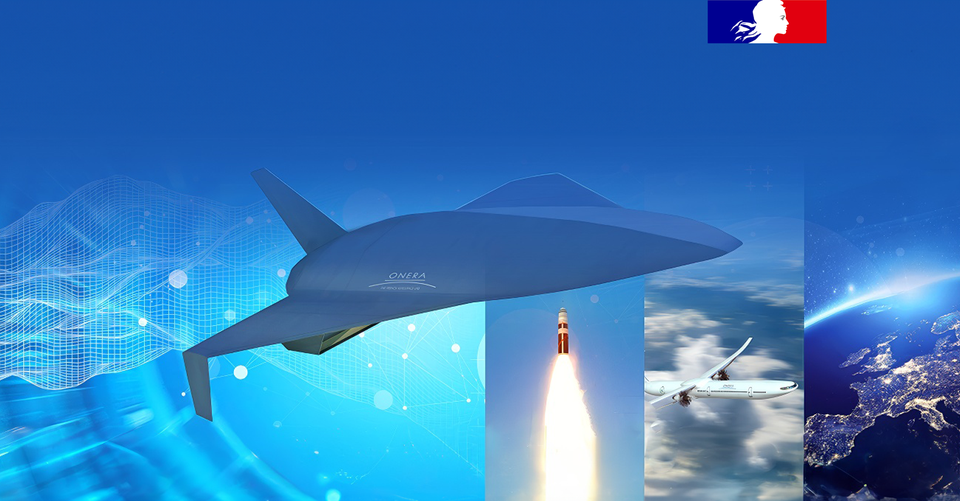
\includegraphics[width=\paperwidth, height=\paperheight]{assets/backgrounds/onera_background.png}}%

\lstset{language=C++,
  frame=single,
  backgroundcolor=\color{white},
  basicstyle=\tiny\ttfamily,
  keywordstyle=\color{blue}\tiny\ttfamily,
  commentstyle=\color{red}\tiny\ttfamily,
  stringstyle=\color{brown}\tiny\ttfamily,
  keepspaces=true,
  showspaces=false,
  tabsize=4
}

\begin{frame}
\Huge
\begin{center}
\textbf{VULKAN}\texttrademark \hspace*{3mm} {\textcolor{orange}{pour le calcul scienfitique}} \\[5mm]
\textcolor{orange}{\textbf{Xavier JUVIGNY}} \\[1cm]

\includegraphics[width=8cm]{images/Onera-bloc-marque.png}
\end{center}
\end{frame}
}

\usebackgroundtemplate{\includegraphics[width=\paperwidth]{assets/backgrounds/paperboard-texture.jpg}}
\begin{frame}
    \frametitle{Plan de l'exposé}
    \tableofcontents
\end{frame}

\section{Présentation générale}

\begin{frame}[fragile]
\frametitle{Historique}

\begin{tabular}{llc}
\textcolor{blue}{\textbf{1992}} & OpenGL (\textcolor{red}{Silicon Graphics}) & $\vcenter{\hbox{
\includegraphics[width=3cm]{images/OpenGL_logo.svg.png}}}$ \\[5mm]
\textcolor{blue}{\textbf{1995}} & DirectX (\textcolor{red}{Microsoft})       & $\vcenter{\hbox{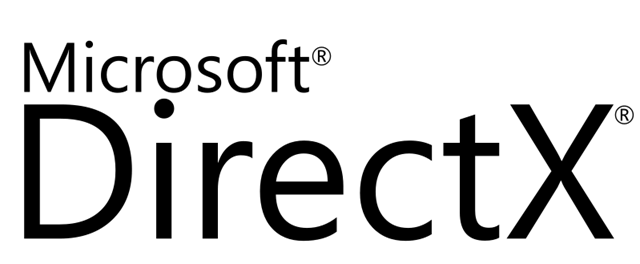
\includegraphics[width=3cm]{images/DirectX_logo.png}}}$ \\[5mm]
\textcolor{blue}{\textbf{2016}} & Vulkan (\textcolor{red}{Khronos Group})    & $\vcenter{\hbox{
\includegraphics[width=3cm]{images/Vulkan_logo.svg.png}}}$
\end{tabular}
\end{frame}

\begin{frame}[fragile]
\frametitle{Vulkan en quelques points}

\begin{itemize}
\item Norme gérée par le consortium industriel Khronos Group (OpenCL, OpenGL, Sycl, slang, WebGL, etc.)
\item Destiné à remplacer OpenGL et OpenGL/ES pour le rendu graphique
\item Supporté par cartes graphiques récentes (\textcolor{red}{$>$ 2016})
\item Exploite architectures modernes des GPGPUs
\item Utilisation multi-c{\oe}urs CPUS pour création images
\item Supporté par principaux OS (\textcolor{DarkGreen}{Windows, Linux, iOS, androïd})
\item API C/C++ proche du hardware des GPGPUs
\item Dernière version 1.3.296 (\textcolor{red}{8 Octobre 2024})
\end{itemize}
\end{frame}

\begin{frame}[fragile]
\frametitle{Objectifs et réalisation}

\begin{exampleblock}{Objectifs}
    \begin{itemize}
    \item Se débarrasser des limitations d'OpenGL
    \item Pouvoir exploiter la puissance totale de la machine
    \end{itemize}
\end{exampleblock}

\begin{alertblock}{Réalisation}
\begin{itemize}
\item Pas d'automate d'état global \\ \refsi{}{} \textcolor{blue}{permet multithreading sur CPUs}
\item Synchronisation CPU--GPU gérée par développeur \\ \refsi{}{} \textcolor{blue}{Optimisation pilote ignorant concurrences mémoires}
\item Mémoire entièrement gérée par développeur \\ \refsi{}{} \textcolor{blue}{Optimisation ressource mémoire GPGPU possible}
\item Vérification erreurs minimale \\ \refsi{}{} \textcolor{blue}{Pas de vérifications dans pilote (optimisation)}
\end{itemize}
\end{alertblock}
\end{frame}

\begin{frame}[fragile]
\frametitle{Langages proposant une API Vulkan}

$\vcenter{\hbox{
\includegraphics[width=1cm]{images/C_Logo.png} 
\includegraphics[width=1cm]{images/cpp_logo.png}}}$

\begin{itemize}
\item Proposés en natif (APIs proches)
\item C++ plus sûr et concis que C
\item \alert{Attention} : la plupart des tutoriaux en C et non en C++
\end{itemize}

$\vcenter{\hbox{
\includegraphics[width=2cm]{images/Python-Logo.png}}}$
\begin{itemize}
\item Plusieurs apis existent mais la plus utiliser : \texttt{\textcolor{blue}{vulkan}} de \textcolor{orange}{\textsl{realitix}}
\item Mais pas de mise à jour depuis plus de sept mois
\end{itemize}

$\vcenter{\hbox{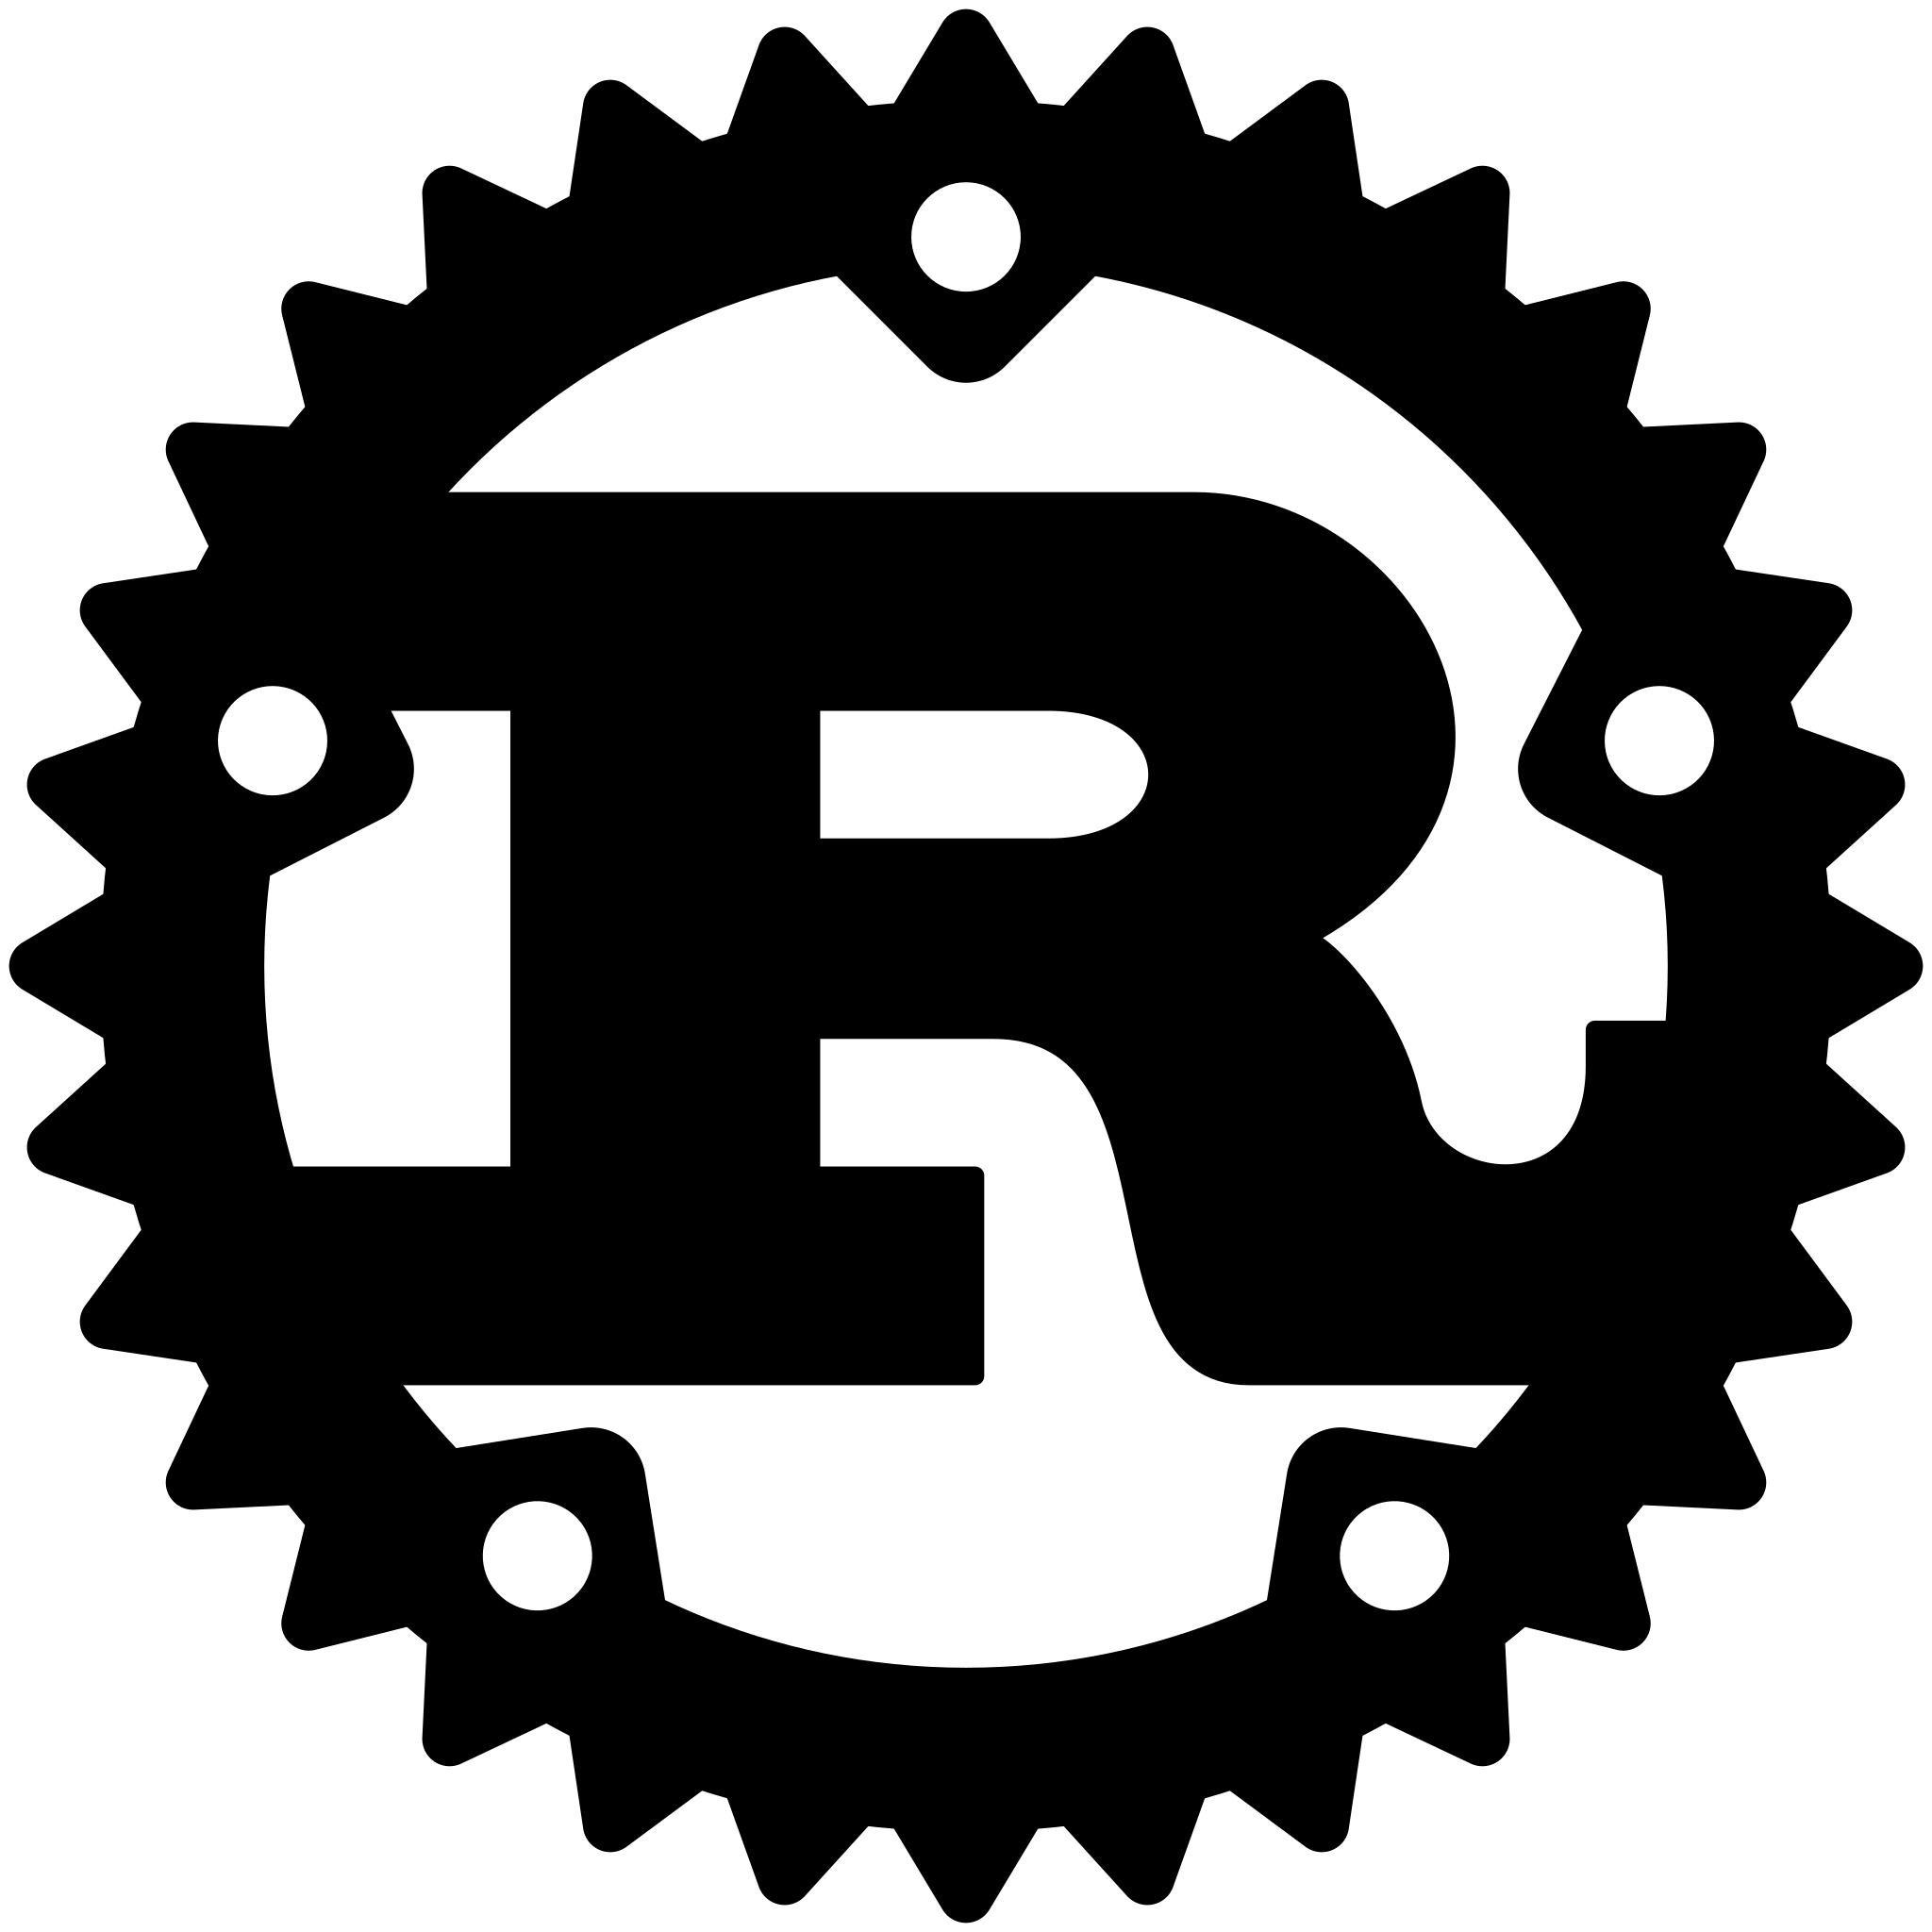
\includegraphics[width=1cm]{images/Rust_programming_language_black_logo.svg.png}}}$
\begin{itemize}
\item \texttt{\textcolor{blue}{vulkano-rs}} : API de référence 
\item Mises à jours régulières
\end{itemize}
\end{frame}

\begin{frame}[fragile]
    \frametitle{Ecosystème Vulkan}
    
    \begin{itemize}
    \item Le \href{https://www.lunarg.com/vulkan-sdk}{kit de développement officiel}, gratuit, développé par LunarG propose de nombreux utilitaires;
    \item \texttt{Vulkan Configurator} (license apache) permet d'outrepasser les composants optionnels définis lors de la création d'une instance dans Vulkan;
    \item Permet de rajouter une couche de validation (avec divers degrés de validation), de trace d'appel, de capture de frame, de diagnostique de crash, etc.
    \item De voir l'environnement Vulkan installé sur la plateforme;
    \item De voir les caractéristiques du GPU gérés par Vulkan ainsi que les extensions associées à ce GPU.
    \item Pour le débogage, voir \href{https://renderdoc.org/}{RenderDoc} qui permet de déboguer des programmes Vulkan.
    \end{itemize}
    
\end{frame}

\section{Présentation de l'API Vulkan}

\begin{frame}[fragile]
\frametitle{Architecture globale}

Vulkan est architecturé pour être facilement extensible pour de nouveaux
hardware et rajouter de nouvelles fonctionnalités.

\begin{figure}[h]
\begin{tikzpicture}
\node[draw, rectangle, fill=green!50!white, drop shadow] at (-2,0) (V) {libvulkan.so};
\node[draw, rectangle, fill=green!50!yellow, drop shadow] at (0,-1.5) (D1) {libvulkan\_intel.so};
\node[draw, rectangle, fill=green!50!yellow, drop shadow] at (-4,-1.5) (D2) {libvulkan\_radeon.so};
\draw[BurntOrange, -{Stealth[blue]}, thick, drop shadow] (V) -- (D1);
\draw[BurntOrange, -{Stealth[blue]}, thick, drop shadow] (V) -- (D2);
\node[draw, rectangle, fill=yellow!50!cyan, drop shadow] at (-4,1.5) (E1) {libext1.so};
\node[draw, rectangle, fill=yellow!50!cyan, drop shadow] at (-2,1.5) (E2) {libext2.so};
\node at (0,1.5) {$\cdots$};
\node at (-1.9,-1.5) {$\cdots$};
\node[draw, rectangle, fill=yellow!50!cyan, drop shadow] at ( 1.5,1.5) (E3) {libextn.so};
\draw[DarkGreen, -{Stealth[BrickRed]}, dashed, thick] (V) -- (E1);
\draw[DarkGreen, -{Stealth[BrickRed]}, dashed, thick] (V) -- (E2);
\draw[DarkGreen, -{Stealth[BrickRed]}, dashed, thick] (V) -- (E3);
\node at (4,0) {\textcolor{red}{\texttt{vk::Instance}}};
\node at (4,-1.5) {\textcolor{red}{\texttt{vk::PhysicalDevice}}};
\node at (4,-2) {\textcolor{red}{\texttt{vk::Device}}};
\node at (4, 1.5) {\textcolor{orange}{Extensions}};
\end{tikzpicture}
\end{figure}

\alert{Note} : Les extensions doivent être validées et "enregistrées" par Khronos Group.
\end{frame}

\begin{frame}[fragile]
\frametitle{Architecture de l'API}

\begin{minipage}{0.335\textwidth}
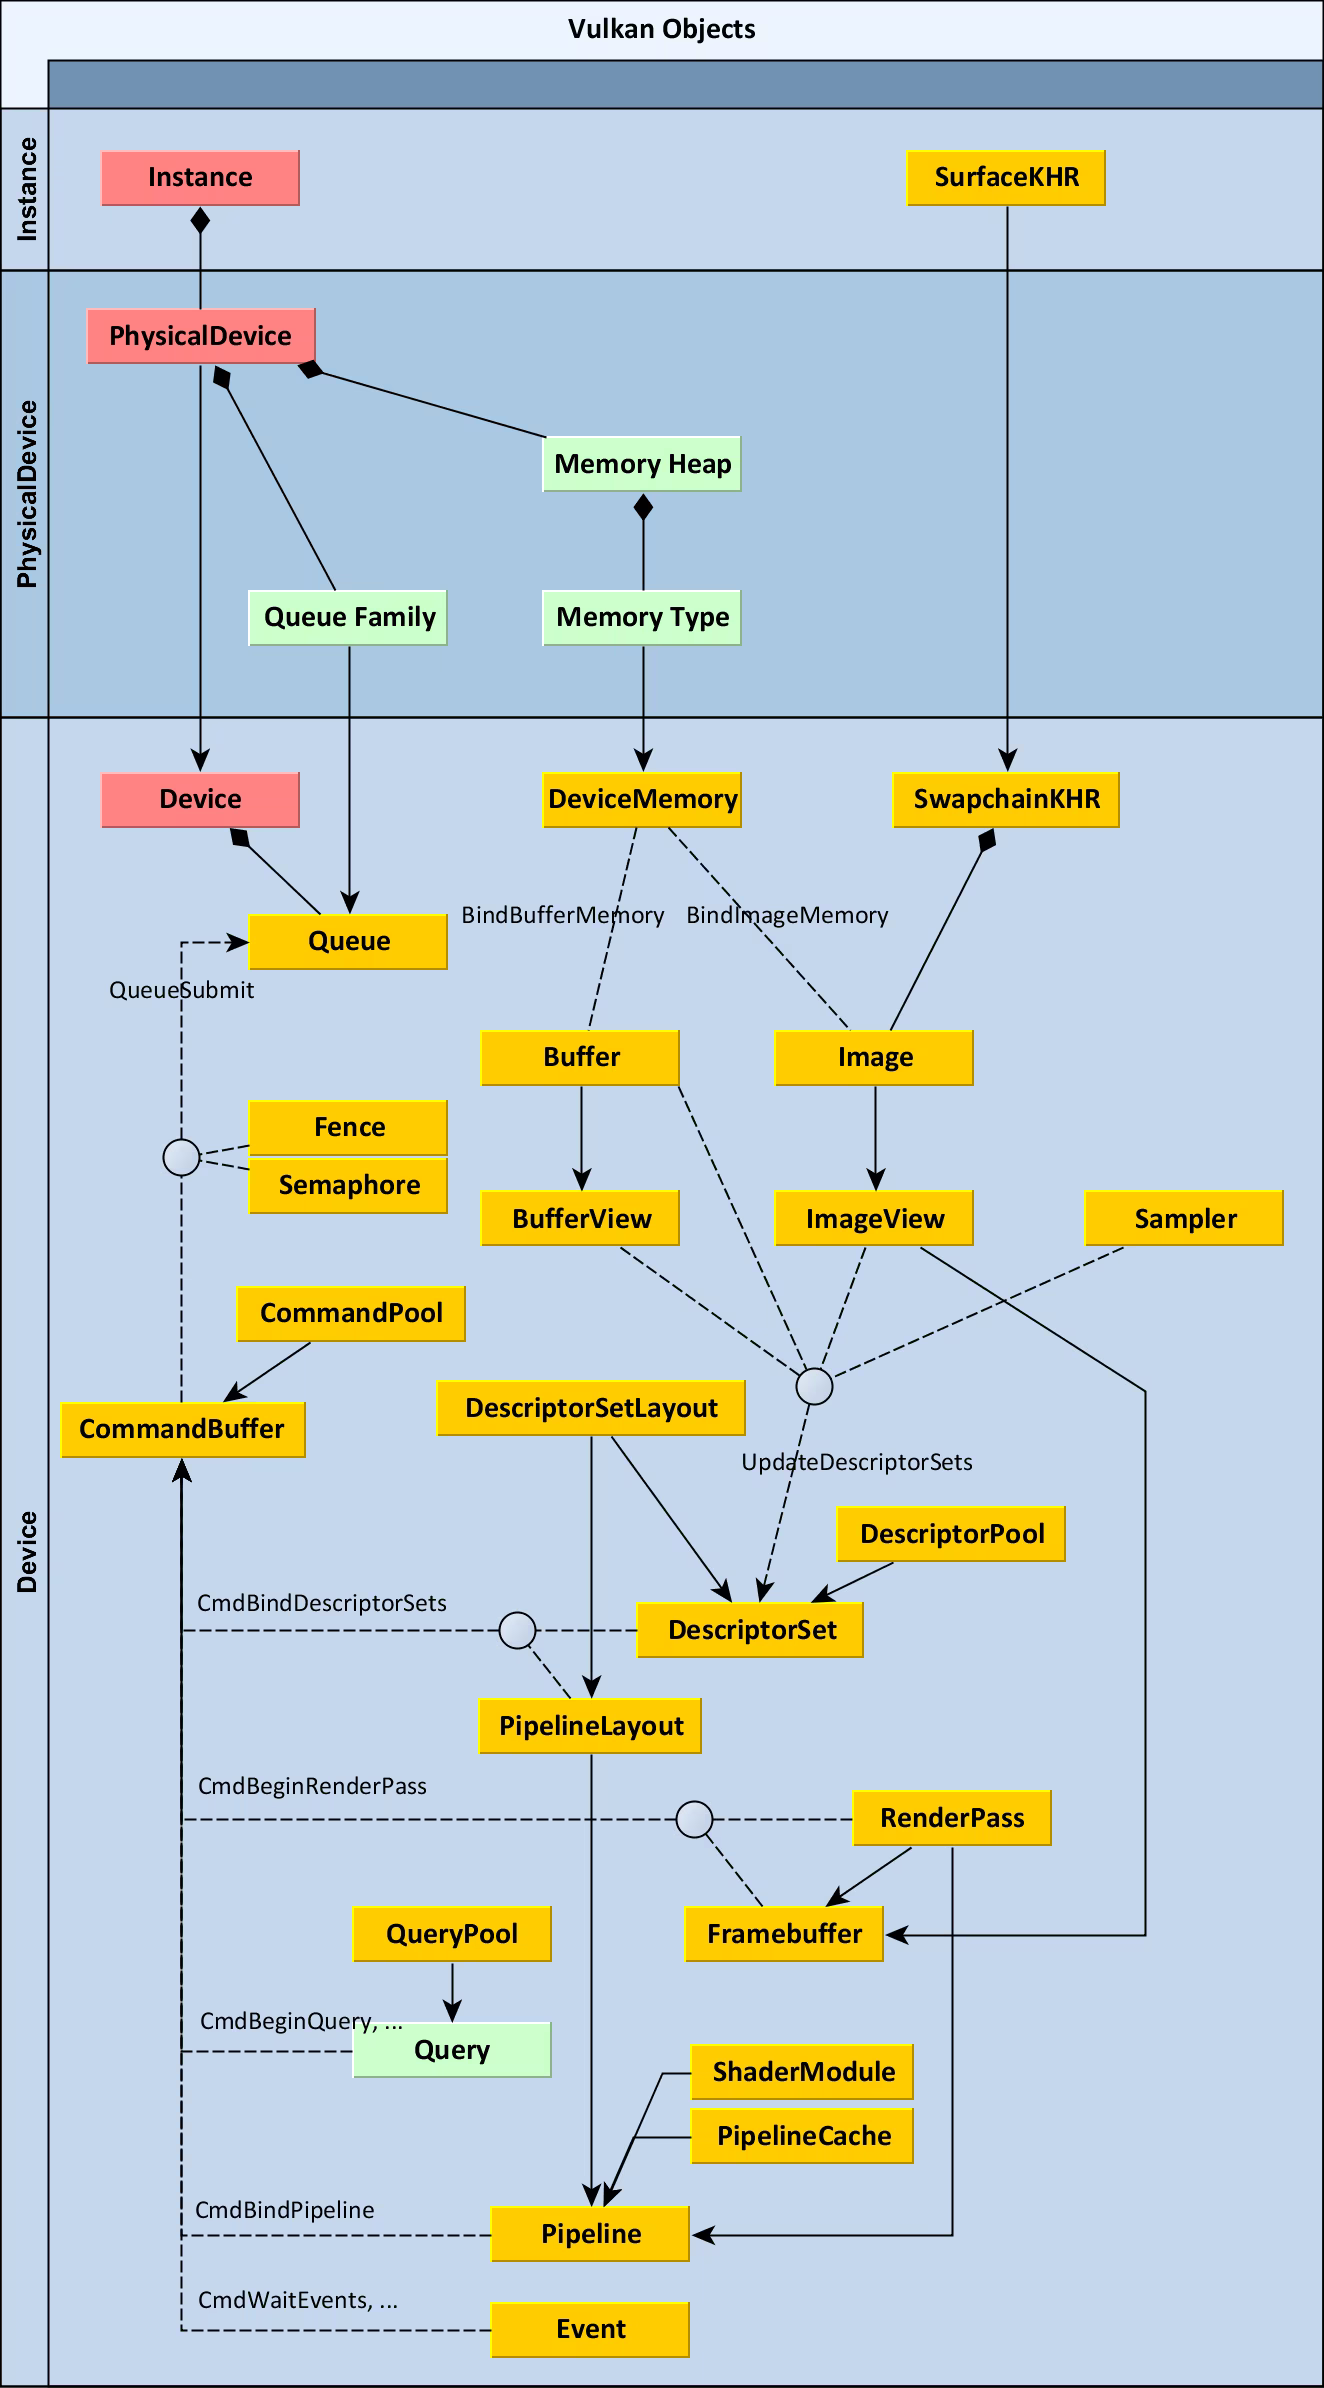
\includegraphics[height=0.75\textheight]{images/Vulkan-Diagram.png}
\centering\href{https://gpuopen.com/learn/understanding-vulkan-objects/}{\scriptsize \textcolor{orange}{\copyright AMD GPUOpen}}
\end{minipage} 
\begin{minipage}{0.65\textwidth}
    {\scriptsize
    \begin{itemize}
    \item $\vcenter{\hbox{\begin{tikzpicture}\node[fill=red!50!white]{\scriptsize Object};\end{tikzpicture}}}$ : Objet principal d'une section (\textcolor{red}{instance obligatoire})
    \begin{itemize}
    \item \scriptsize\textcolor{blue}{Permet création autres objets de la section}
    \end{itemize}
    \item $\vcenter{\hbox{\begin{tikzpicture}\node[fill=green!50!white]{\scriptsize Object};\end{tikzpicture}}}$ : Objet non typé uniquement indexé par un entier
    \begin{itemize}
    \item \scriptsize \textcolor{blue}{Appartient et indexé par un objet}
    \end{itemize}
    \item $\vcenter{\hbox{\begin{tikzpicture}\draw[->, >= triangle 45,black] (0,0) -- (2em,0);\end{tikzpicture}}}$ représente l'ordre de création
    \item $\vcenter{\hbox{\begin{tikzpicture}\draw[{Diamond[]}-,black] (0,0) -- (2em,0);\end{tikzpicture}}}$ représente une composition
    \item $\vcenter{\hbox{\begin{tikzpicture}\draw[dashed,black] (0,0) -- (2em,0);\end{tikzpicture}}}$ représente une autre relation
    \end{itemize}
    }
\end{minipage}
\end{frame}

\subsection{Les shaders}

\begin{frame}[fragile]
\frametitle{Les shaders}

\begin{itemize}
\item Introduits en Mai 1988 par Pixar dans logiciel \textcolor{orange}{Renderman};
\item Change comportement de certaines étapes de rendus par ses propres programmes;
\item Introduit dans OpenGL et Direct3D vers 2001;
\item Personnaliser certaines étapes du rendu d'OpenGL/DirectX;
\item Plusieurs langages développés proches du C/C++ :
      \begin{itemize}
      \small
      \item \href{https://registry.khronos.org/OpenGL/specs/gl/GLSLangSpec.4.60.pdf}{\textcolor{NavyBlue}{OpenGL shading language}} ou \textcolor{BrickRed}{GLSL}
      \item \href{https://microsoft.github.io/hlsl-specs/specs/hlsl.pdf}{\textcolor{NavyBlue}{DirectX High-Level Shader Language}} ou \textcolor{BrickRed}{HLSL}
      \end{itemize}
\item Les différents shaders existants :
     \begin{itemize}
     \small
     \item \textcolor{NavyBlue}{Tessellation} : Subdivise un élément du maillage
     \item \textcolor{NavyBlue}{Vertex}   : Projette un sommet 3D vers écran.
     \item \textcolor{NavyBlue}{Geometry} : Modifie géométrie d'un polygone
     \item \textcolor{NavyBlue}{Fragment} : calcule couleur d'un pixel
     \item \textcolor{NavyBlue}{Compute} : Effectue des calculs parallèles complexes
     \item \textcolor{NavyBlue}{Raytracing} : calcule intersection rayon--triangle
     \end{itemize}
\end{itemize}
\end{frame}

\begin{frame}[fragile]
\frametitle{Spécification des shaders avec Vulkan}

\begin{itemize}
\item Avec OpenGL, compilation des shaders se fait par l'API;
\item Pour portabilité, obligé avec OpenGL de livrer application avec source des shaders
\item Avec Vulkan, langage machine binaire SPIRV
\item Facile à transformer en langage machine natif du GPGPU
\item compilateurs externes existent indépendant de Vulkan
\item Permettent de compiler shaders GLSL ou HLSL en SPIRV
\item Exemple de compilateurs permettant de compiler des shaders écrits en GLSL ou en HLSL en SPIRV :
  \begin{itemize}
  \item \textcolor{NavyBlue}{glslang}
  \item \textcolor{NavyBlue}{glslc}
  \end{itemize}
\item API Vulkan permet de charger directement du SPIV pour les shaders
\end{itemize}
\end{frame}

\begin{frame}[fragile]
\frametitle{Le compute shader}
\lstset{style=customglsl}

\begin{itemize}
\item Permet d'effectuer des calculs complexes
\item Préciser la version du langage utiliser dans votre code :
\begin{lstlisting}
#version 450
\end{lstlisting}
\item Organisation des threads sur grille 1D, 2D ou 3D
\item Notion groupe de travail $\equiv$ OpenCL ou bloc Cuda
\item A définir en C++ mais aussi dans le shader !

\begin{lstlisting}
#define WORKGROUP_SIZE 32
layout (local_size_x=WORKGROUP_SIZE, 
        local_size_y=WORKGROUP_SIZE, local_size_z=1) in;
\end{lstlisting}
\end{itemize}
\end{frame}

\begin{frame}[fragile]
\lstset{style=customglsl}
\frametitle{Passer des paramètres à un shader}

\begin{itemize}
\item Impossible de passer directement paramètres dans \textcolor{blue}{\texttt{main}}.
\item Pour passer des paramètres, on peut passer :
\begin{itemize}
    \item Des constantes pour de simples valeurs en entrée :
\begin{lstlisting}
layout( push_constant ) uniform Constants {
    vec2 dimensions;
} constants;    
\end{lstlisting}    
    \item Des buffer uniformes pour un groupe de valeurs (pouvant être structurées ) en entrée :
\begin{lstlisting}
layout(binding=2, set=0) uniform CameraProperties {
    mat4 viewInverse; mat4 projInverse; vec4 lightPos;
} cam;    
\end{lstlisting}
    \item Des buffers pour des collections de valeurs :
\begin{lstlisting}
layout(std140, binding = 0) buffer buf {
    vec4 imageData[];
};    
\end{lstlisting}
\end{itemize}
\end{itemize}
\end{frame}

\begin{frame}[fragile]
\frametitle{Repérer la position d'un thread sur la grille de threads}
\lstset{style=customglsl}

\begin{itemize}
\item \textbf{Rappel} : chaque thread positionné sur grille 1D/2D ou 3D à l'aide d'un n-uple d'entiers
\item La grille est subdivisé en blocs de threads (groupe en GLSL);
\item Possibilité de connaître le positionnement global du thread exécutant notre code :
\begin{lstlisting}
float x = float(gl_GlobalInvocationID.x) / float(WIDTH);
float y = float(gl_GlobalInvocationID.y) / float(HEIGHT);
\end{lstlisting}
\item Possibilité de connaître le positionnement dans un bloc du thread exécutant notre code :
\begin{lstlisting}
sharedA[gl_LocalInvocationID.y][gl_LocalInvocationID.x] = A[row * N + (k * 16 + gl_LocalInvocationID.x)];
\end{lstlisting}
\end{itemize}
\end{frame}

\subsection{L'API côté hôte}

\begin{frame}[fragile]
\frametitle{Les étapes de création d'une application Vulkan}

\underline{Structure "fixe"}
\begin{itemize}
\item Définir un contexte Vulkan
\item Choisir le(s) périphérique(s) physique(s) disponible(s)
\item Définir un périphérique logique représentant le(s) périphérique(s) physique(s)
\item Choisir une ou plusieurs queues d'exécution selon le(s) type(s) de traitement
\item Décrire la structure sous-jacente en mémoire représentée par les buffers utilisées dans les shaders
\item Créer des réservoirs pour la création de buffers de commandes et de pipeline 
\item Créer le(s) buffer(s) de commande
\item Créer le(s) pipeline(s) associés au(x) buffer(s) de commande.
\end{itemize}
\end{frame}

\begin{frame}[fragile]
\frametitle{Les étapes de création d'une application Vulkan (suite)}

\underline{Structure "dynamique"}
\begin{itemize}
\item Créer des buffers en choisissant le type de mémoire dans lequel réserver;
\item Transférer éventuellement des données de l'hôte vers le périphérique;
\item Associer des buffers avec un numéro de binding (et éventuellement de set) utilisés dans les shaders;
\item Exécuter un buffer de commande (ou plusieurs en parallèle).
\end{itemize}
\end{frame}

\begin{frame}[fragile]
\frametitle{Les couches logicielles (Layers)}

Création d'un contexte : on peut rajouter des couches logicielles.

\begin{block}{Couche logicielle (Layer)}
\begin{itemize}
\item Certaines étapes de l'exécution ont des points d'interruption
\item On peut y brancher  nos propres couche(s) logicielle(s)
\item Possibilité d'enchaîner  plusieurs fonctions d'interruption
\item \textcolor{NavyBlue}{\bf Exemples} :
\begin{itemize}
\item Débogueur pour intercepter et afficher les problèmes détectés par Vulkan;
\item Sauvegarder des frames à des moments spécifiques
\end{itemize}
\item Possible de demander la liste des couches logicielles préexistantes
 à l'exécution de l'application.
 \item Possibilité de programmer propres couches 
 (voir \href{https://renderdoc.org/vulkan-layer-guide.html}{\textcolor{blue}{la documentation fournie par renderdoc}})
\end{itemize}
\end{block}
\end{frame}

\begin{frame}[fragile]
\frametitle{Les extensions}

Création d'un contexte : on peut rajouter des extensions 

\begin{exampleblock}{Extensions}
\begin{itemize}
\item Des fonctionnalités peuvent être rajoutées dynamiquement :
\item Deux types de fonctionnalités : celles liées à l'environnement et l'autre à chaque périphérique
\item \textcolor{NavyBlue}{\bf Exemple}:
\begin{itemize}
    \item Ecrire sur un type de surface donnée (Metal, Wayland, X11, Windows)
    \item Des fonctionnalités pour supporter l'accélération RTX
\end{itemize}
\item Pour chaque fonctionnalités disponibles, possibilité d'avoir des pointeurs sur les fonctions associées à l'extension
\item \textbf{\textcolor{BrickRed}{Note 1}} : Contrairement aux layers, rajout d'une extension doit être approuvée par Khronos Group
\item \textbf{\textcolor{BrickRed}{Note 2}} : Certains layers sont associés avec une extension donnée (par exemple pour le déboggage d'applications Vulkan)
\end{itemize}
\end{exampleblock}
\end{frame}

\begin{frame}[fragile]
\frametitle{\textcolor{BrickRed}{\bf Exemple} : Rajout d'un outil de validation/débogage}

\lstset{style=customcpp}
\begin{lstlisting}[language=C++]
std::vector<const char*> enabled_layers{},enabled_ext{};
auto layer_properties=vk::enumerateInstanceLayerProperties();
bool has_validation_layer_type = false;
for (auto prop : layer_properties)
{
  if (strcmp("VK_LAYER_KHRONOS_validation",prop.layerName)==0) 
    has_validation_layer_type = true;
}// for (auto prop : ....)
if (has_validation_layer_type)
  enabled_layers.push_back("VK_LAYER_KHRONOS_validation");
\end{lstlisting}

\begin{lstlisting}[language=C++]
auto extensions=vk::enumerateInstanceExtensionProperties();
for (auto prop : extensions)
{
  if (strcmp(VK_EXT_DEBUG_UTILS_EXTENSION_NAME,prop.extensionName) == 0)
  {
    enabled_ext.push_back(VK_EXT_DEBUG_UTILS_EXTENSION_NAME);
  }
}
\end{lstlisting}

\end{frame}

\begin{frame}[fragile]
\frametitle{Création d'un contexte Vulkan}
Lors de la création d'un contexte Vulkan, il faut :
\begin{itemize}
\item Scanner les couches logicielles disponibles pour le driver Vulkan disponible sur la machine
\item Sélectionner les couches logicielles désirées (chaînes de caractère)
\item Scanner les extensions disponibles pour le driver Vulkan
\item Sélectionner les extensions logicielles désirées (chaînes de caractère)
\item Décrire votre application
\item Créer le contexte à partir des données précédentes.
\end{itemize}
\end{frame}

\begin{frame}[fragile]
\frametitle{Création du contexte}

\lstset{style=customcpp}
\begin{lstlisting}[language=C++]
vk::ApplicationInfo application_info;
application_info.setApiVersion(vk::ApiVersion13)
                .setPApplicationName("Computing shader")
                .setApplicationVersion(0)
                .setPEngineName("Computing engine")
                .setEngineVersion(0);

vk::InstanceCreateInfo create_info;
create_info.setPApplicationInfo(&application_info)
           .setPEnabledLayerNames(enabled_layers)
           .setPEnabledExtensionNames(enabled_ext);

vk::Instance instance = vk::createInstance(create_info);
\end{lstlisting}
\end{frame}

\begin{frame}[fragile]
\frametitle{Choisir son périphérique}

\begin{itemize}
\item Plusieurs périphériques compatibles avec Vulkan :
  \begin{itemize}
  \item le CPU (via une couche llvm)
  \item le GPU interne au CPU 
  \item le GPU dédié
  \item etc.
  \end{itemize}
\item Vulkan chargera un driver spécifique selon le périphérique choisit;
\item On doit donc choisir un (ou des) périphérique(s);
\item Pour cela, il faut interroger chaque périphérique géré par Vulkan pour sélectionner selon le besoin de l'application.
\end{itemize}
\end{frame}

\begin{frame}[fragile]
    \frametitle{Choisir son périphérique (suite)}


\begin{itemize}
\item Récupérer tous les périphériques compatibles Vulkan :
\lstset{style=customcpp}
\begin{lstlisting}[language=C++]
auto devices = instance.enumeratePhysicalDevices();
for (auto device : devices) { ...
\end{lstlisting}
\item Pour chaque périphérique :
\begin{itemize}
\item \textcolor{NavyBlue}{\lstinline|dev.getFeatures()|}  décrit 
fonctionnalités fines disponibles sur périphérique :
test débordements de buffer ? Tracer droites d'épaisseur $>1$ ? etc.
\item \textcolor{NavyBlue}{\lstinline|dev.getProperties()|} décrit  propriétés hardware : dédié ou intégré ? taille limite
des entités (buffer, constantes, textures, etc.), nom, versions vulkan supporté, etc.
\item \textcolor{NavyBlue}{\lstinline|dev.getMemoryProperties()|} décrit les types mémoires supportées et leurs capacités :
mémoire partagée avec CPU, mémoire dédiée, texture, constante, etc.
\item \textcolor{NavyBlue}{\lstinline|dev.enumerateDeviceExtensionProperties()|} : les extensions
disponibles ($\neq$ extensions de l'instance)
\item \textcolor{NavyBlue}{\lstinline|dev.enumerateDeviceLayerProperties()|} : les layers
disponibles \\($\subset$ layers de l'instance)
\end{itemize}
\end{itemize}
\end{frame}

\begin{frame}[fragile]
\frametitle{Création d'un périphérique logique}

\begin{itemize}
\item Pour contrôler le(s) périphérique(s) réel(s), on doit créer un périphérique
\textcolor{blue}{logique} qui nous servira d'API;
\item Le contrôle des GPGPUs se fait par un système de queue de commande;
\item Il existe plusieurs types de queues de commande :
\begin{itemize}
    \item Une queue dédiée au transfert de mémoire CPU $\Longleftrightarrow$ GPU ?
    \item Une queue dédiée au calcul uniquement ?
    \item Une queue dédiée au graphisme ?
    \item Une queue pour le calcul et le graphisme ?
    \item etc.
    \end{itemize}
\item On doit donc spécifier le(s) type(s) de queues de commande qu'on veut utiliser
\item Mais aussi les extensions du périphérique qu'on veut utiliser;
\item Et enfin les fonctionnalités fines qu'on souhaite utiliser.
\end{itemize}
\end{frame}

\begin{frame}[fragile]
\frametitle{Création des buffers}

\textcolor{BurntOrange}{\textbf{\underline{Deux types de buffers}} :}
\begin{itemize}
\item \textcolor{NavyBlue}{\texttt{Uniform buffer}} : Pour stocker un ensemble de données
en entrée (lecture seule) pour les shaders
\item \textcolor{NavyBlue}{\texttt{Storage buffer}} : Buffer stockant un ensemble de valeurs en lecture/écriture
modifiable par les shaders
\end{itemize}
\textcolor{BurntOrange}{\underline{Mêmes protocoles pour les gérer (mais fonctions parfois $\neq$)}} :
\begin{itemize}
\item Création du buffer (descriptif) : 
\begin{itemize}
    \scriptsize
\item Nombre d'octets nécessaire qu'on va devoir réserver ?
\item Pour quel usage ? Uniform ? Storage ? Encore/Décodage vidéo ? etc.
\item Mode d'accès : exclusif (à une queue) ou en concurrence
\end{itemize}
\item Rechercher la mémoire adéquate avec la description du buffer et les caractéristiques voulues par le programmeur
\item Allouer la mémoire
\item Relier la mémoire avec le buffer (bind)
\item Copier données mémoire hôte vers mémoire GPU (optionnel)
\end{itemize}
\end{frame}

\begin{frame}[fragile]
\frametitle{Association des buffers avec les shaders}

\textcolor{BrickRed}{\textbf{\underline{Mécanisme complexe mais souple} !}}
\begin{itemize}
    \small
\item Pour chaque ensemble (set) dans les shaders, décrire
l'organisation mémoire attendue pour chaque shader dans un \texttt{DescriptorSetLayout}.
\item Préparer un réservoir de descripteur avec max descripteurs pouvant être alloués
\item Allouer les descripteurs à partir de l'organisation mémoire qu'on a décrit : prépare
des objets de réceptions des buffers qu'on va utiliser dans chaque shader
\item Puis autant de fois qu'on veut, affecter des buffers aux différents objets créés par un descripteur
\end{itemize}
\end{frame}

\begin{frame}[fragile]
\frametitle{Déclaration du Pipeline}

\begin{tikzpicture}
\node[drop shadow,fill=white] (PL) {\scriptsize\texttt{PipelineLayout}};
\node[drop shadow,fill=white, above=1cm of PL] (DSL) {\scriptsize\texttt{DescriptorSetLayout}};
\node[drop shadow,fill=white, right=2cm of PL] (P) {\scriptsize\texttt{Pipeline}};
\draw[-{Stealth[NavyBlue]}] (DSL) -- (PL);
\draw[-{Stealth[NavyBlue]}] (PL) -- (P);
\node[drop shadow,fill=white, above=2cm of P] (SM) {\scriptsize\texttt{ShaderModule}};
\node[drop shadow,fill=LightCyan, above right=2cm of P] (PC) {\scriptsize\texttt{PipelineCache}};
\node[drop shadow,fill=yellow, right=2cm of P] (RP) {\scriptsize\texttt{RenderPass}};
\draw[-{Stealth[NavyBlue]}] (SM) -- (P);
\draw[-{Stealth[NavyBlue]}] (PC) -- (P);
\draw[-{Stealth[NavyBlue]}] (RP) -- (P);
\end{tikzpicture}

\begin{itemize}
\item Les GPUs calculent une image en plusieurs étapes dont l'ordonnancement est
fixe : \textcolor{BrickRed}{Pipeline} graphique.
\item Certaines étapes optionnelles et personnalisables (shaders, transferts)
\item Vulkan demande de définir nos pipelines graphiques en :
\begin{itemize}
\small
\item Précisant les types de shader devant être exécutés
\item Chargeant et associant les shaders utilisés
\item Précisant leurs points d'entrée (en général \texttt{\textcolor{blue}{main}})
\item Précisant la description des ensembles de descripteurs utilisés
\end{itemize}
\end{itemize} 
\end{frame}

\begin{frame}[fragile]
\frametitle{Déclaration du buffer de commande}
\begin{center}
\begin{tikzpicture}
\node[drop shadow,fill=white] (CB) {\scriptsize\texttt{CommandBuffer}};
\node[drop shadow,fill=white, left=2cm of CB] (P) {\scriptsize\texttt{Pipeline}};
\node[drop shadow,fill=yellow, above=1cm of CB] (E) {\scriptsize\texttt{Event}};
\node[drop shadow,fill=white, above left=1cm of CB] (CP) {\scriptsize\texttt{CommandPool}};
\draw[-{Stealth[NavyBlue]}] (P) -- (CB);
\draw[DarkGreen, -{Stealth[NavyBlue]}] (E) -- (CB);
\draw[-{Stealth[NavyBlue]}] (CP) -- (CB);
\end{tikzpicture}
\end{center}

Pour déclarer un buffer de commande, il faut :
\begin{itemize}
\small
\item Déclarer la queue d'exécution qu'on veut utiliser
\item Créer un réservoir de buffer de commande utilisant cette queue;
\item Allouer à partir de ce réservoir un ou plusieurs buffers de commande;
\item Pour chaque buffer de commande :
\begin{itemize}
\small
\item Débuter l'enregistrement des commandes qu'on devra exécuter
\item Au moins relier un pipeline et des descripteurs au buffer de commande;
\item Puis préciser la répartition des threads pour le shader de calcul;
\item Enfin terminer l'enregistrement.
\end{itemize}
\end{itemize}
\end{frame}

\begin{frame}[fragile]
\frametitle{Exécution du buffer de commande}

\begin{center}
\begin{tikzpicture}
\node[drop shadow,fill=white] (CB) {\scriptsize\texttt{CommandBuffer}};
\node[right=2cm of CB] (X) {\scriptsize$\circ$};
\node[drop shadow,fill=white, right=4cm of CB] (Q) {\scriptsize\texttt{Queue}};
\node[drop shadow,fill=white, above right=1cm of CB] (F) {\scriptsize\texttt{Fence}};
\node[drop shadow,fill=white, right=1cm of F] (S) {\scriptsize\texttt{Semaphore}};
\draw[-{Stealth[BrickRed]}] (CB) -- (X);
\draw[-{Stealth[BrickRed]}] (X) -- (Q);
\draw[dashed, -{Stealth[NavyBlue]}, BrickRed] (F) -- (X);
\draw[dashed, -{Stealth[NavyBlue]}, BrickRed] (S) -- (X);
\end{tikzpicture}
\end{center}
    
\begin{itemize}
\item L'exécution d'un buffer de commande est asynchrone.
\item Il faut prévoir au moins une barrière pour la synchronisation
\item Les étapes à suivre sont donc :
\begin{itemize}
\small
\item Préparer une soumission d'un ou plusieurs buffers de commande;
\item Créer au moins une barrière de synchronisation (Fence)
\item Soumettre notre soumission à la queue avec la barrière de Synchronisation
\item Puis attendre la fin de la synchronisation 
\item Enfin détruire la barrière de synchronisation
\item On récupère les données sur l'hôte en mappant un buffer mémoire de sortie
\end{itemize} 
\end{itemize}

\end{frame}

\begin{frame}[fragile]
\frametitle{Test performance sur un ensemble de mandelbrot}

\underline{\textbf{\textcolor{BrickRed}{Ensemble de mandelbrot}}}

\begin{itemize}
\item On considère la suite récursive complexe : \\
$
\left\{
    \begin{array}{lcl}
        z_{0} & = & 0 \\
        z_{n+1} & = & z_{n}^{2} + c
    \end{array}
\right.
$
où $c\in\mathbb{C}$ choisie.
\item On étudie la convergence/divergence de cette suite selon $c$;
\item Si $\exists N$ tel que $\vert z_{N} \vert >= 2$, la suite diverge;
\item Dans certaines zones dans disque $\rho < 2$, la suite converge;
\item Sinon impossible montrer convergence/divergence de la suite;
\item Image représente partie plan complexe : à chaque pixel $p$ correspond un $c$;
\item Si suite "converge", $p$ devient noir, sinon couleur dépend du premier $N$ tel que 
$\vert z_{N}\vert >=2$.
\end{itemize}

\end{frame}

\begin{frame}[fragile]
\frametitle{Test de performance sur le calcul de l'ensemble de mandelbrot}

\textcolor{BrickRed}{But} : Calculer en simple précision l'ensemble de mandelbrot
sur une image $3200\times2400$ pixels avec 512 itérations max.

\begin{itemize}
\item Test "idéal" car très peu d'accès à la mémoire par rapport à la charge de calcul;
\item Permet de tester le maximum qu'on peut tirer d'un GPU intégré sans mémoire dédiée.
\end{itemize}

\begin{tikzpicture}
\node[draw=none,shade,blur shadow={shadow xshift=0ex,shadow yshift=0ex, shadow blur radius=1ex},inner sep=0pt]
{\scriptsize
\begin{tabular}{|c|c|c!{\color{blue}\vrule\hspace*{0.1mm}\vrule}c|c|c!{\color{red}\vrule\hspace*{0.1mm}\vrule}c|} \hline
\rowcolor{LightCyan}
Processeur & c{\oe}urs & Tps & GPGPU & c{\oe}urs & Tps & rapport \\  \arrayrulecolor{orange}\specialrule{.1em}{.05em}{.05em}\arrayrulecolor{black}
Intel i5 11th gen. & 4(8) & 795 & Intel IRIS $X^{e}$ & 80 & 43 & 18.5 \\ \hline
Intel i7 11th gen. & 8(16) & 617 & GeForce RTX 3060 & 3584 & 8 & 77 \\ \hline
\end{tabular}
};
\end{tikzpicture}

Temps exprimé en millisecondes.

\end{frame}

\section{API utilisant Vulkan}

\begin{frame}[fragile]
\frametitle{Comment éviter toute cette complexité ?}

\begin{itemize}
\item Vulkan très puissant mais complexe à mettre en {\oe}uvre;
\item Existe des librairies dédiées au calcul avec Vulkan
\item Exemple \href{https://github.com/KomputeProject/kompute}{Kompute}
\item \alert{Mais}
\begin{itemize}
\item Petit projet\dots
\item Encore en version beta
\item Manque encore quelques fonctionnalités
\item Mais permet de tester un produit matrice-matrice en Vulkan !
\end{itemize}
\item Autres projets simplifiant Vulkan (encore non testé !) : 
\begin{itemize}
\item \href{https://github.com/jgbit/vuda}{VUDA} : coder Vulkan en Cuda API!
\item \href{https://github.com/Tencent/ncnn}{NCNN} : Neural network interface
\item \href{https://github.com/vinjn/awesome-vulkan}{Site centralisant les projets vulkan}
\end{itemize}
\end{itemize}
\end{frame}

\begin{frame}[fragile]
\frametitle{Produit matrice-matrice}

\begin{itemize}
\item Produit  plein : $C = A.B$ avec $A,B,C\in\mathbb{R}^{N\times N}$
\item Pour faciliter la vérification du résultat :
\begin{itemize}
\item $A = U_{A}.V_{A}^{t}$ avec $U_{A},V_{A}\in\mathbb{R}^{N}$;
\item $B = U_{B}.V_{B}^{t}$ avec $U_{B},V_{B}\in\mathbb{R}^{N}$;
\item $C = U_{A}.V_{A}^{t}.U_{B}.V_{B}^{t} = (V_{A}|U_{B}) U_{A}.V_{B}^{t}$
\end{itemize}
\end{itemize}

\underline{\textcolor{BrickRed}{dimension 1024}}

\begin{tikzpicture}
\node[draw=none,shade,blur shadow={shadow xshift=0ex,shadow yshift=0ex, shadow blur radius=1ex},inner sep=0pt]
{\scriptsize
\begin{tabular}{|c|c|c!{\color{blue}\vrule\hspace*{0.1mm}\vrule}c|c|c|} \hline
\rowcolor{LightCyan}
Processeur & c{\oe}urs & GFlops & GPGPU & c{\oe}urs & GFlops \\  \arrayrulecolor{orange}\specialrule{.1em}{.05em}{.05em}\arrayrulecolor{black}
Intel i5 11th gen. & 4(8) & 180 & Intel IRIS $X^{e}$ & 80 & 55 \\ \hline
Intel i7 11th gen. & 8(16) & 250 & GeForce RTX 3060 & 3584 & 330 \\ \hline
\end{tabular}
};
\end{tikzpicture}

\underline{\textcolor{BrickRed}{dimension 4096}}

\begin{tikzpicture}
    \node[draw=none,shade,blur shadow={shadow xshift=0ex,shadow yshift=0ex, shadow blur radius=1ex},inner sep=0pt]
    {\scriptsize
    \begin{tabular}{|c|c|c!{\color{blue}\vrule\hspace*{0.1mm}\vrule}c|c|c|} \hline
    \rowcolor{LightCyan}
    Processeur & c{\oe}urs & GFlops & GPGPU & c{\oe}urs & GFlops \\  \arrayrulecolor{orange}\specialrule{.1em}{.05em}{.05em}\arrayrulecolor{black}
    Intel i5 11th gen. & 4(8) & 195 & Intel IRIS $X^{e}$ & 80 & 60 \\ \hline
    Intel i7 11th gen. & 8(16) & 255 & GeForce RTX 3060 & 3584 & 330 \\ \hline
    \end{tabular}
};
\end{tikzpicture}    

\begin{itemize}
\item \alert{Des optimisations encore possible dans le shader !}
\item \textcolor{NavyBlue}{Remarque 1} : Sur RTX, Cublas affiche 638 GFlops !
\item \textcolor{NavyBlue}{Remarque 2} : C++ : produit par bloc multithreadé 27GFlops!
\end{itemize}
\end{frame}

\section{Conclusion}

\begin{frame}[fragile]
\frametitle{Conclusions}

\makeatletter
\def\@shadowbox#1{%
  \setbox\@fancybox\hbox{\fcolorbox{black}{cyan!15}{#1}}%
  \leavevmode\vbox{%
    \offinterlineskip
    \dimen@=\shadowsize
    \advance\dimen@ .5\fboxrule
    \hbox{\copy\@fancybox\kern-.5\fboxrule\lower\shadowsize\hbox{%
      \vrule \@height\ht\@fancybox \@depth\dp\@fancybox \@width\dimen@}}%
    \vskip-\dimen@
    \moveright\shadowsize\vbox{%
      \hrule \@width\wd\@fancybox \@height\dimen@}}}
\makeatother

\shadowbox{Vulkan}
\begin{itemize}
\item permet d'écrire des codes puissants
\item Mais plus adapté au graphisme qu'au calcul
\item Préférable d'utiliser OpenCL que Vulkan 
\item Mais Vulkan permet aussi de faire du raytracing hardware
\item Interaction entre Vulkan et OpenCL possible
\item Interaction OpenCL-Vulkan pour raytracing acoustique
\end{itemize}

\shadowbox{KCompute}
\begin{itemize}
\item Grande simplification du code;
\item Mais encore en développement;
\item Continuer à tester...
\end{itemize}
\end{frame}
\end{document}
